\chapter{Методы статического межпроцедурного анализа программ} \label{chapt1}


\section{Используемая терминология}

Одной из основных задач, возникающих при создании программного продукта любой сложности, является обеспечение его качества. Для определения соответствия разрабатываемого программного продукта критериям качества в состав жизненного цикла программного обеспечения включают стадии или процессы верификации и валидации программных средств \cite{gost-12207, gost-34.601}. Верификация, согласно \cite{lipaev-zakaz}~--- это процесс для определения, выполняет ли программный комплекс и его компоненты требования, наложенные на них в последовательных этапах жизненного цикла комплекса программ. В водопадной модели жизненного цикла программного обеспечения (ПО) стадия верификации и тестирования непосредственно следует за стадией реализации программного продукта \cite{waterfall} (рис. \ref{pic:lifecycle-waterfall}); в итеративной модели стадия тестирования также следует за реализацией, однако циклически повторяется по мере разработки системы. Ряд методологий, например, разработка через тестирование \cite{tdd}, подразумевает интеграцию тестирования с процессом разработки. 

\begin{figure}[h]
   \centering
   
\includegraphics[width=\linewidth]{lifecycle-waterfall}
   \caption{Жизненный цикл программы в каскадной модели разработки и место в нём тестирования}\label{pic:lifecycle-waterfall}
\end{figure}

Целью верификации является подтверждение соответствия конечного программного продукта предопределённым эталонным требованиям, для чего осуществляется обнаружение, регистрация и устранение дефектов, внесённых при разработке или модификации программных комплексов и компонентов или требований к ним. Для повышения результативности издержек верификация должна быть объединена как можно раньше с процессами проектирования, производства и сопровождения \cite{lipaev-zakaz}.

Вместе с тем, отдельной стадии тестирования, как правило, недостаточно для построения безопасного комплекса с низким количеством дефектов. В связи с эти для построения безопасных программных продуктов используются специальные методологии разработки, в которых требования к безопасности и обеспечению высокого качества программного продукта предъявляются на каждой из стадий разработки. Одной из наиболее известных методологий безопасной разработки ПО является Microsoft Security Development Lifecycle (Microsoft SDL, жизненный цикл защищённой разработки Microsoft) \cite{ms-sdl}. Диаграмма жизненного цикла ПО согласно данной методологии представлена на рисунке \ref{pic:ms-sdl}. 

\begin{figure}[h]
   \centering
   \includegraphics[width=\linewidth]{ms-sdl}
   \caption{Жизненный цикл защищённой разработки Microsoft (Microsoft SDL)}\label{pic:ms-sdl}
\end{figure}

Данная методология предполагает использование 17 различных практик, применяемых на различных стадиях создания программного продукта, для повышения качества и надёжности разрабатываемого ПО:

\begin{enumerate}
 \item \textit{Обучение участников разработки} основам информационной безопасности и поддержка их знаний в актуальном состоянии. Необходимые навыки включают безопасное проектирование, моделирование угроз, безопасную разработку, тестирование безопасности и обработку конфиденциальных данных.
 \item \textit{Разработка требований безопасности} и их анализ. Определение требований безопасности на ранних стадиях позволяет осуществлять их реализацию неотъемлемо от разработки программного продукта.
 \item \textit{Создание стандартов качества}, устанавливающих минимально допустимый уровень безопасности и конфиденциальности. Установка требований качества на начальной стадии создания ПО улучшает восприятие рисков безопасности и стимулирует устранение дефектов безопасности в процессе разработки. Кроме того, стандарты качества задаются для каждой стадии создания ПО, что позволяет контролировать процесс появления и устранения дефектов.
 \item \textit{Оценка рисков безопасности и конфиденциальности} определяет, какие элементы системы должны подвергаться дополнительным видам тестирования и верификации, и какому риску они могут подвергнуться в процессе эксплуатации.
 \item \textit{Определение требований проектирования} включает создание проектных спецификаций возможностей безопасности и конфиденциальности, с которыми непосредственно взаимодействует пользователь, а также описаний методик разработки функциональных возможностей с учётом требований безопасности.
 \item \textit{Анализ атак} позволяет уменьшить риск предоставления атакующему возможностей для эксплуатации потенциально слабого места или уязвимости и включает ограничение доступа к системным сервисам, применение принципа наименьших привилегий и использование многослойной защиты.
 \item \textit{Моделирование угроз} позволяет структурированно учитывать, документировать и обсуждать влияние требований безопасности на разработки, что, в свою очередь, позволяет рассмотрение проблем безопасности на уровне компонента или приложения.
 \item \textit{Использование одобренных инструментов} подразумевает определение и использование списка инструментов разработки, одобряемого консультантом по вопросам безопасности, и их возможностей проверок безопасности, таких как опции и предупреждения компилятора или компоновщика.
 \item \textit{Избежание небезопасных функций} означает запрет на использование потенциально небезопасных и устаревших функций и интерфейсов с их заменой на безопасные альтернативы и проверки кода на их использование.
 \item \textit{\textbf{Статический анализ}} предоставляет возможность масштабируемого аудита безопасности программного кода и соблюдение политик безопасной разработки.
 \item \textit{\textbf{Динамический анализ}} подразумевает верификацию времени выполнения. Он необходим для проверки соответствия функциональности программы проектной.
 \item \textit{\textbf{Нечёткое тестирование (fuzz testing)}} проверяет программу на устойчивость к повреждённым, случайным или злонамеренно искажённым данным.
 \item \textit{Обзор векторов атак} представляет собой пересмотр модели угроз  и векторов атак по окончании разработки кода и необходим для проверки отсутствия появления или устранения обнаруженных новых векторов атак в результате изменений системы в процессе разработки.
 \item \textit{План реагирования на инциденты} перечисляет персонал, ответственный за оперативное устранение обнаруживаемых уязвимостей, и содержит планы обслуживания кода, внешнего по отношению к команде разработчиков.
 \item \textit{Окончательная проверка безопасности} является последовательной проверкой всех аспектов безопасности продукта перед его выпуском и проводится с целью идентификации и устранения дефектов и уязвимостей, внесённых на различных стадиях разработки ПО.
 \item \textit{Архив выпусков продукта} используется для обслуживания ПО после его выпуска и включает в себя, помимо непосредственно программного кода, все спецификации, двоичные файлы, модели угроз, документацию, лицензии, планы оперативного реагирования и прочую информацию, которая может понадобиться для обслуживания выпущенного ПО.
 \item \textit{Инспекции кода} специалистами в области безопасности подвергаются критические с точки зрения безопасности компоненты разрабатываемой системы. Инспекция кода проводится с целью проверки корректности работы с конфиденциальными данными и поиска дефектов при реализации криптографических алгоритмов. 
\end{enumerate}

Как можно заметить, три практики предусматривают непосредственное использование специализированных инструментальных средств тестированя и верификации. Другие существующие практики безопасной разработки, такие как TSP-Secure (Team Software Process for Secure Development) \cite{tsp}, также включают использование инструментальных анализаторов исходного или бинарного кода.

Целью инструментального анализа кода программы является определение наличия в нём \textit{ошибок}. В широком смысле под ошибкой (или \textit{дефектом}) понимается неправильность, погрешность или искажение объекта или процесса \cite{lipaev-soft-eng}. Анализаторы обычно оперируют более узким понятием дефекта, понимая его как описанный класс свойств программного кода, приводящих к нарушению требований к качеству программе. Данное определение подразумевает описание свойства программы, которое необходимо анализатору для поиска дефекта. Для многих видов дефектов, встречаемых при разработке программ, существуют описания и классификация. Наиболее известными среди них являются каталоги Common Weaknesses Enumeration (CWE) \cite{cwe}, Computer Emergency Readiness Team (CERT) \cite{cert-org}, Motor Industry Software Reliability Association (MISRA) \cite{misra}. Существуют также отраслевые и проектные стандарты, включающие список возможных нарушений, такие как JSF C++ Coding Standards \cite{jsf}.

Поскольку автоматизированный поиск дефектов производится с использованием формальных методов, для поиска дефектов обычно недостаточно описания. На основе описания класса дефектов строится \textit{критерий дефектности}~--- формальное описание класса дефекта или его подмножества, позволяющее производить автоматический поиск. Для автоматизации поиска используется программа, называемая \textit{анализатором}. Критерий дефектности обычно формулируется в терминах \textit{модели анализатора}~--- описания анализатора и его принципа работы, учитывающего особенности его реализации. Задачей анализатора обычно является построение внутренних структур данных на основе кода программы, проверка полученных структур на соответствие заданному критерию дефектности и выдача диагностических сообщений в случае обнаружения соответствия.

Срабатывания анализатора и отсутствие срабатывания можно разделить на корректные и ложные. Срабатывание анализатора является \textit{корректным (true positive, TP)}, если отчёт анализатора указывает на действительно присутствующий в коде программы дефект. Срабатывание анализатора является \textit{ложным (false positive, FP)}, если программный код на самом деле не содержит дефекта, указанного в отчёте анализатора. Отсутствие срабатывание анализатора является \textit{корректным (true negative, TN)}, если программный код, на котором анализатор не выдал диагностическое сообщение, действительно является корректным. Отсутствие срабатывания анализатора является \textit{некорректным (false negative, FN)}, или \textit{пропуском}, если анализатор не выдал диагностическое сообщение при анализе программного кода, содержащего дефект.

Ряд срабатываний анализатора являются положительными с точки зрения соответствия правилу поиска, однако по-каким либо причинам код невозможно изменить так, чтобы он соответствовал правилу кодирования. Такая ситуация может возникнуть, например, при необходимости поддерживать стандартизированный программный интерфейс (например, JNI~--- Java Native Interface, Posix-функции). Такие срабатывания принято классифицировать отдельной категорией~--- \textit{\todo{придумать перевод} Intentional}.

Основных источников ложных срабатываний несколько. Во-первых, в силу различных ограничений анализатору недоступна вся возможная информация о программе и её окружении. Многие анализаторы производят анализ программы по частям, что дополнительно уменьшает объём доступной анализатору информации. Во-вторых,  структуры данных анализатора зачастую строятся с упрощением, поскольку хранение и использование всей возможной информации о программе требует большого количества ресурсов, а время анализа должно быть ограничено. В-третьих, источником ложных срабатываний может являться недостаточно однозначная спецификация дефекта, которая может включить образец поиска в список дефектных, хотя он таковым не является. В-четвёртых, некорректная реализация проверки (ошибка при реализации или неучёт каких-либо условий) также может приводить к ложным срабатываниям.

Обычно с целью повысить независимость проверок друг от друга и отделить их от реализации моделирования языка программирования анализатор архитектурно разделяют на:

\begin{enumerate}
 \item фронтэнд~--- часть, отвечающую за разбор исходного файла и построение базовых структур данных (синтаксическое дерево, таблица идентификаторов и др.). Зачастую в качестве фронтэнда используется уже существующий компилятор, который строит все структуры данных сам.
 \item ядро анализатора отвечает за реализацию \todo{алгоритма} и моделирование операторов языка
 \item проверяющие модули непосредственно реализуют проверки, используя данные, предоставляемые ядром анализатора, а также предоставляют ядру анализатора информацию, влияющую на моделирование.
\end{enumerate}


% Здесь написать об абстрактной интерпретации (см. книгу драконов).

\section{Метод анализа программ с помощью символьного выполнения} \label{sect1_1}
В данной работе исследуется метод символьного выполнения \cite{king76}, применяемый для анализа путей выполнения программ. Этот метод подразумевает абстрактное движение по путям программы, имитирующее её выполнение в~зависимости от~входных данных, сопровождающееся изменением состояния программы в~различных точках. Суть метода символьного выполнения заключается в~разбиении множества входных данных на~классы эквивалентности, что позволяет оперировать при~анализе не~отдельными входными значениями (число которых может быть очень большим и~экспоненциально растёт в~зависимости от~количества входных аргументов) и~их перебором, а~целыми классами эквивалентности, число которых может оказаться и~не конечным, но не~превышает общее количество комбинаций отдельных входных значений. Однако, как~правило, количество классов эквивалентности комбинаций входных данных оказывается значительно ниже числа всех возможных комбинаций входных данных, что резко увеличивает возможности анализатора по обработке путей выполнения.

Основной алгоритм символического выполнения \cite{king76} заключается в~следующем.
\begin{enumerate}
 \item При~старте анализа функции входные значения её аргументов и~внешних по отношению к~ней переменных неизвестны, т.~е. они потенциально могут принимать любые значения. Начальное состояние является корневым узлом специального графа~--- дерева выполнения программы.
 \item Каждой неизвестной величине назначается абстрактное значение, называемое символьным значением.
 \item Обработка операторов языка изменяет значения переменных программы, т.~е. их символьные значения. Считается, что над символьными значениями уже определён необходимый набор операций для~вычисления новых символьных значений на~основе уже имеющихся. Выполнение каждого оператора добавляет узел к~дереву выполнения программы с~входящим ребром от~предыдущего оператора.
 \item При~обработке условных операторов в~дерево выполнения программы добавляется не~один, а~два узла: в~первом узле условие выполняется, во втором~--- нет. Совокупность условий, при~которых достижим данный узел графа выполнения программы, определяет класс эквивалентности входных данных программы или функции. Таким образом, каждый лист дерева выполнения программы соответствует классу эквивалентности входных данных, которая приводит программу в~конечное состояние, обозначаемое данным листом. 
 \item Обычно каждое из условий, определяющих класс эквивалентности входных данных, можно представить в~виде уравнения или неравенства. В~результате наложения на~путь выполнения программы нескольких условий в~соответствие каждому классу эквивалентности входных данных ставится система уравнений или неравенств. Решениями этих систем уравнений являются множества реальных значений входных величин, при~которых будут выполнены ветви выполнения программы. Если система является несовместной, т.~е. не~имеет ни~одного решения, то путь выполнения, соответствующий этой системе, недостижим.
 \item Анализатор производит обход всех путей получившегося дерева выполнения с~целью поиска ситуаций, которые могли бы трактоваться как~некорректное поведение. В~случае обнаружения такой ситуации анализатор сообщает о~дефекте и~при этом указывает набор условий, при~выполнении которых программа проявит некорректное поведение.
\end{enumerate}

Данный алгоритм можно рассмотреть на~следующем примере. Пусть имеется следующая программа чтения из файла на~языке C:

\begin{verbatim}
     1  int test(int a, int b) {
     2    FILE *f = fopen("file.txt");
     3    int result;
     4    fscanf(f, "%d", &result);
     5    fclose(f);
     6    if (a == 0 && b > 2) {
     7      fclose(f);
     8      return 0;
     9    }
    10    return result;
    11  }
\end{verbatim}

В~результате выполнения этой программы будут достижимы три конечных состояния с~уравнениями $a \neq 0, b \in [INT\_MIN, INT\_MAX]$; $a = 0, b \leqslant 2$; $a = 0, b > 2$. Соответствующий граф представлен на~рис.~\ref{pic:sample-exec}.

\begin{figure}
   \centering
   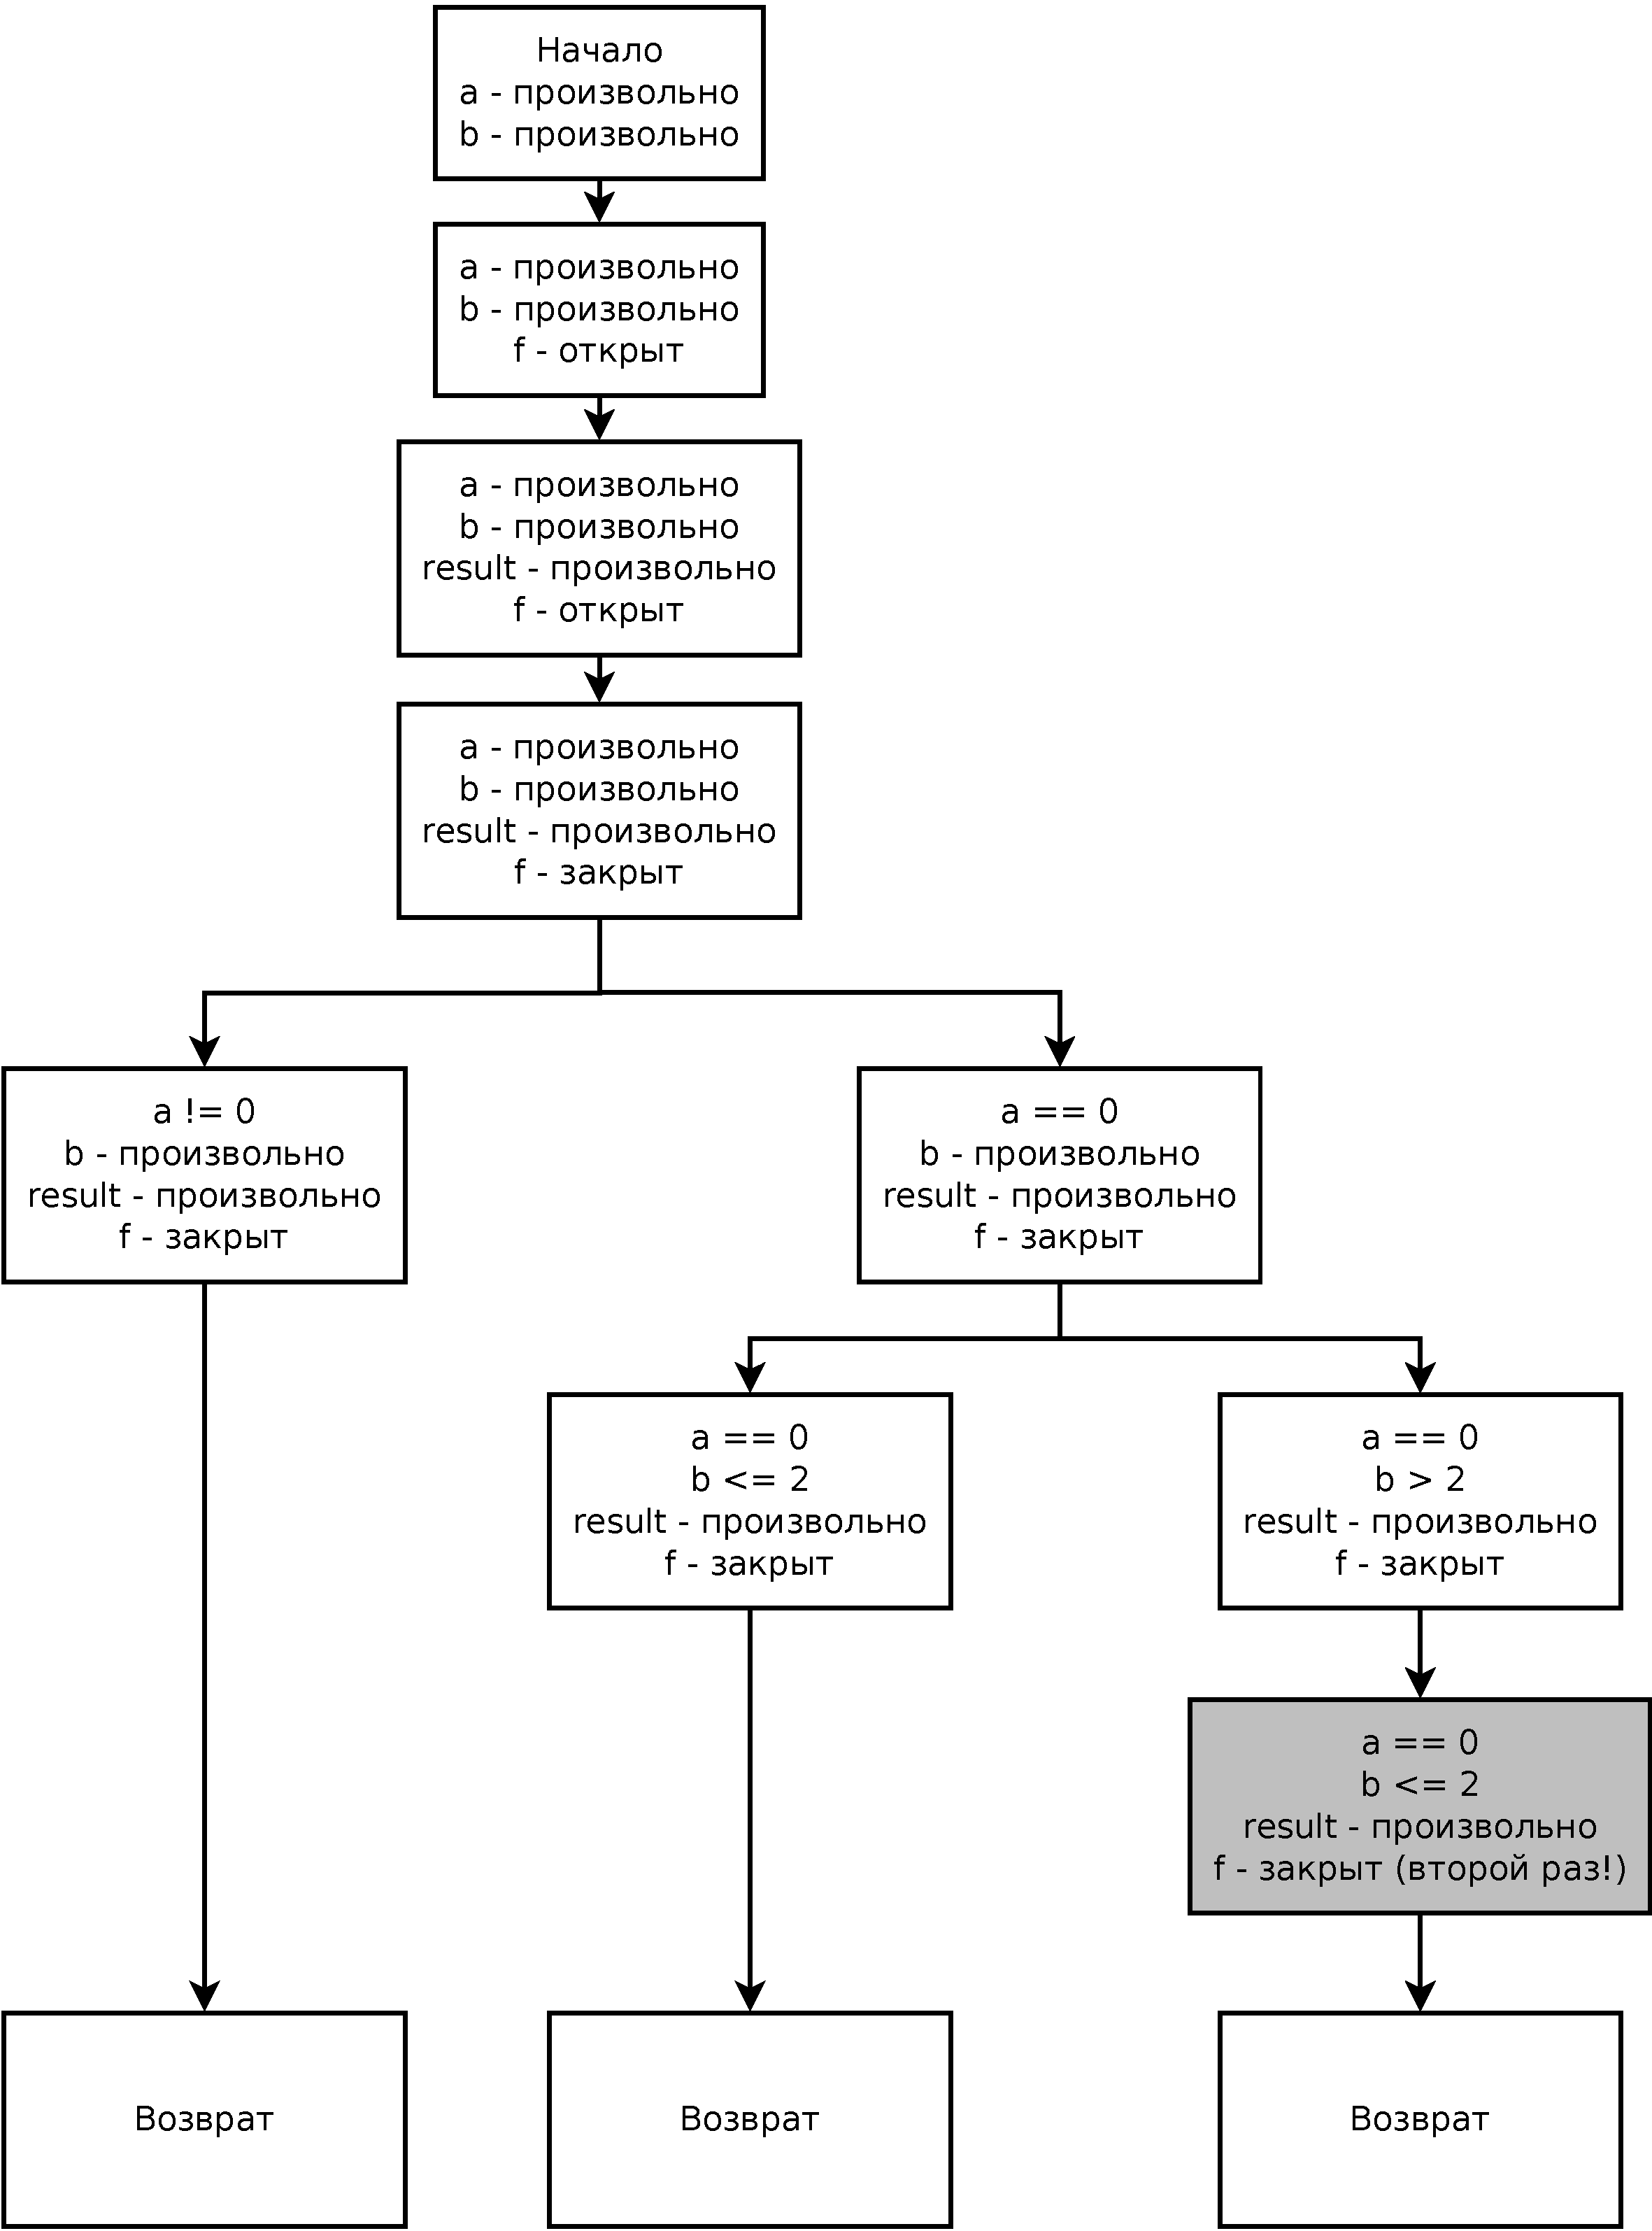
\includegraphics[width=0.9\linewidth]{article-1-symexec-sample.pdf}
   \caption{Граф выполнения программы чтения из файла}\label{pic:sample-exec}
\end{figure}

В~результате получены три пути с~соответствующими ограничениями. Теперь анализатор просматривает каждый из этих путей и~обнаруживает дефект: на~одном из путей файл \texttt{f} закрывается дважды, что приводит к~неопределённому поведению. Этому пути соответствует система $a = 0, b > 2$. Таким образом дефекту сопоставляется множество условий, при~котором он проявляется при~выполнении программы.

Основным преимуществом метода символьного выполнения является простота и~очевидность концепции, на~которой он основан: метод использует идею <<симуляции>> выполнения программы, так, как~это делает программист. Метод символьного выполнения получил распространение не~только в~инструментах статического, но и~смешанного анализа: так, хорошо зарекомендовали себя инструменты, использующие подход concolic testing \cite{concolic}  (символьно-конкретное~--- concrete+symbolic). Concolic testing~--- это метод поиска дефектов, осуществляющий генерацию тестовых данные, при~использовании которых программа проявляет некорректное поведение, на~основе символьного выполнения.

Наряду с~преимуществами, метод имеет ряд недостатков. Так, существует проблема экспоненциального роста количества проходимых путей (path explosion), приводящая к~проблемам с~масштабируемостью метода. Есть также проблемы при~моделировании циклов, поскольку зачастую количество итераций цикла точно неизвестно~--- оно также является символьной величиной. Тем не~менее, метод символьного выполнения активно применяется, в~том числе, целым набором широко используемых инструментов анализа программ. Таким образом, разработка подходов для~улучшения данного метода является актуальной и~практически важной задачей.

Основные проблемы масштабируемости метода связаны с~двумя факторами.
\begin{enumerate}
 \item При~моделировании циклов время анализа линейно зависит от~количества итераций, проходимых программой при~выполнении цикла. Даже если число итераций известно, но велико, анализ программы выполняется длительное время, резко возрастающее при~наличии в~программе вложенных циклов. При~использовании смешанного анализа обычно эту проблему анализом выполнения программы для~установления реального количества итераций. При~статическом анализе наиболее распространённым решением является ограничение количества итераций циклов каким-либо максимальным константным значением. Этот подход позволяет ограничить время анализа, однако не~решает проблему роста времени анализа при~наличии вложенных циклов. Кроме того, это ограничение приводит к~потере точности моделирования, что, в~свою очередь, приводит к~ложным срабатываниям или отсутствию срабатываний в~тех случаях, когда они ожидаются.
 \item Время анализа быстро растёт при~использовании межпроцедурного анализа.
\end{enumerate}

Отличие межпроцедурного анализа (МПА) от~внутрипроцедурного (ВПА) заключается в~том, что анализатор позволяет использовать доступные определения пользовательских функций для~моделирования эффектов их вызовов. МПА используется для~решения двух основных проблем, связанных с~использованием внутрипроцедурного анализа. Во-первых, межпроцедурный анализ позволяет определить эффект, оказываемый на~состояние программы в~результате вызова из анализируемой функции другой функции. В~отсутствие межпроцедурного анализа вызов функции можно моделировать либо самостоятельно (с помощью спецификаций эффектов), либо приближённо. Первый подход, как~правило, используется для~функций, эффекты которых специфицированы. Таковы, например, функции различных публичных интерфейсов взаимодействия. Наиболее распространено такое моделирование для~Posix API, встречаются также реализации, моделирующие вызовы Windows API. Кроме того, хорошими кандидатами на~специфицирование являются функции, принадлежащие стандартной библиотеке языка, поскольку она, как~правило, стандартизирована, реже~--- функции других распространённых библиотек (например, STL и~др.).

Во-вторых, в~случае, если полная спецификация функции недоступна, при~внутрипроцедурном анализе может использоваться приближённое моделирование. В~этом случае считается, что вызов функции может произвести любые действия с~данными, которые доступны внутри функции (для языков, имеющих операции арифметики с~указателями, например, C/C++, в~общем случае можно считать, что программа может модифицировать любые данные), и~вернуть произвольное значение. Для~уточнения эффектов может использоваться анализ атрибутов доступной декларации функции, например, информация о~модификаторах типов аргументов функции, атрибуты аргументов и~самой функции. Так, например, функция, объявленная с~GNU-атрибутом \texttt{\_\_attribute\_\_((pure))}, не~имеет прав на~изменение глобальной памяти и~аргументов, а~функция с~атрибутом \texttt{\_\_attribute\_\_((noreturn))} никогда не~вернёт управление в~вызывающую функцию. Могут также использоваться различные эвристики. Вместе с~тем, приближённое моделирование может решить проблему анализа лишь частично. Из-за невозможности оценки влияния вызова на~состояние программы анализатор может сделать некорректные выводы о~текущем состоянии выполнения программы, что может привести как~к~ложным срабатываниям анализатора (ошибка первого рода), так и~к отсутствию срабатывания в~условиях, когда анализатор должен выдавать диагностическое предупреждение (ошибка второго рода).

\todo{написать про виды чувствительностей}

\section{Межпроцедурный анализ для метода символьного выполнения}

Межпроцедурный анализ при использовании метода символьного выполнения обычно выполняется с использованием метода встраивания \cite{???}. Метод встраивания заключается в моделировании операторов вызываемой функции оператор за оператором, в порядке, определяемом потоком управления функции. В начале моделирования вызова устанавливается соответствие имён, внутренних для вызываемой функции, и имён в контексте вызывающей функции: так, значениями формальных параметров вызываемой функции становятся значения её фактических аргументов в вызывающей функции, объектам ключевых слов \texttt{this} или \texttt{self} ставится в соответствие объект, вызов метода которого моделируется, и т.~д.. Затем функция моделируется так же, как и вызывающая, формируя дальнейший путь выполнения. По окончании моделирования вызова значение, возвращаемое оператором \texttt{return}, становится значением, возвращаемым функцией в контексте вызывающей функции, после чего продолжается моделирование вызывающей функции.

Метод встраивания достаточно прост в реализации и, кроме того, является естественным для смешанного анализа, поскольку соответствует непосредственному выполнению анализируемой программы. Его дополнительное преимущество заключается в сохранении всех видов чувствительностей анализа:

\begin{enumerate}
 \item этот метод сохраняет контекстную чувствительность, поскольку на значения переменных при моделировании вызова функции накладываются ограничения, существующие в вызывающей функции;
 \item метод сохраняет чувствительность к пути выполнения, поскольку \todo{???}
 \item метод сохраняет чувствительность к потоку \todo{???}
\end{enumerate}


Однако метод встраивания имеет недостаток, связанный с масштабируемостью: каждый раз при моделировании вызова функции она анализируется заново, в различных контекстах. Это приводит к большим расходам как процессорного времени, затрачиваемого на анализ, так и к расходам памяти, поскольку информацию, получаемую при моделировании вызова на каждом его шаге, и зачастую необходимую для последующего анализа, необходимо сохранять в памяти. В результате сравнения времени анализа с использованием межпроцедурного анализа методом встраивания и без использования межпроцедурного анализа были получены значения времени \todo{time-1} и \todo{time-2} (для тестирования использовался программный комплекс Clang Static Analyzer). Эти данные показывают заметное увеличение времени анализа. При этом время анализа зависело от размера исходного файла следующим образом: \todo{графики}.

Поскольку нашей задачей является сохранение всех видов чувствительности анализа


\todo{!!!}


Таким образом, нашей задачей является построение такого метода межпроцедурного анализа для метода символьного выполнения, который будет обладать следующими свойствами:

\begin{enumerate}
 \item сохранение всех видов чувствительности анализа, т.~е. метод МПА должен сохранять контекстную чувствительность, чувствительность к пути и чувствительность к потоку;
 \item высокая масштабируемость: разрабатываемый метод должен позволять анализ крупных программных систем за приемлемое время;
 \item достаточная точность анализа: реализация разрабатываемого метода не должна уступать методу встраивания в количестве корректных срабатываний (и, по возможности, не допускать пропусков дефектов) и в отношении количества корректных срабатываний к общему количеству срабатываний.
\end{enumerate}


\section{Улучшения метода символьного выполнения}

Низкая масштабируемость метода символьного выполнения в его оригинальном описании является известной проблемой, и многие исследователи пытались решить её различными способами. Для уменьшения времени анализа и улучшения покрытия, а также для решения других возникающих проблем, предлагались различные решения.

Часть исследователей пыталась решить проблему роста количества путей, уменьшая количество ветвлений состояния программы. В этом отношении интересны работы \cite{state-merge, state-merge-securware}. В этих работах получаемые в результате выполнения пути выполнения программы вместе с соответствующими им классами эквивалентности по возможности объединяются в один сразу после ветвления. В результате объединения ветвей выполнения анализатором рассматривается не отдельное состояние программы в процессе выполнения, а суперпозиция состояний, получаемых на различных путях выполнения программы. Применение данного подхода уменьшает количество анализируемых путей программы, что позволяет снизить время анализа, однако, поскольку при анализе одного объединённого пути  анализируются несколько фактических, анализ происходит без потери анализатором покрытия кода. 

Использование событийного подхода при программировании приложения создаёт ряд проблем для анализа программы, поскольку, во-первых, обычно код, отвечающий за низкоуровневую обработку событий находится не в приложении, а в системной или прикладной библиотеке, а, во-вторых, порядок и состав приходящих событий не может быть определён заранее. Это приводит к комбинаторному взрыву вариантов выполнения программы. Попытка решения этой проблемы представлена, в частности, в \cite{anand-thesis}.

Метод символьного выполнения имеет ряд недостатков, связанных с анализом циклов в программе. Во-первых, количество итераций цикла может быть заранее неизвестным, и представлять собой символьное значение, не вычисляемое в константное при произвольном множестве значений входных данных. В этом случае невозможно предсказать или рассчитать количество итераций цикла, которое необходимо проанализировать без потери точности и полноты анализа. Во-вторых, время анализа цикла растёт в зависимости от количества итераций (как правило, линейно), и при значительном количестве итераций цикла анализ программы становится слишком длительным. Эта проблема становится серьёзнее в случае наличия вложенных циклов, для которых время анализа растёт в зависимости от количества итераций каждого из циклов, а также при использовании межпроцедурного анализа, который может значительно увеличивать длину пути выполнения каждой итерации цикла.

Поскольку циклические конструкции являются неотъемлемой частью любой программы, проблемы, связанные с анализом циклов, привлекали исследовательский интерес. Кроме того, циклы обычно используются для обработки контейнерных типов и для работы с рекурсивными структурами данных, поэтому без решения данной проблемы невозможно построить анализатор, пригодный для промышленного использования. Для решения проблем моделирования циклов предлагались и используются различные методы и эвристики. 

Первый подход использует моделирование заранее фиксированного количества итераций цикла. Этот подход достаточно хорошо работает в случае, если потенциальное количество итераций невелико, однако проблемы производительности, связанные с вложенными циклами, данный подход решает хуже, и резкий рост времени анализа в этом случае сохраняется, хотя время анализа и ограничивается сверху. Кроме того, ограничение количества итераций приводит к уменьшению покрытия путей программы, что, в свою очередь, может привести к пропуску дефектов. Данный подход применяется, в частности, в Clang Static Analyzer. Другие подходы к анализу циклов предполагают вычисление фиксированной точки цикла или некоторого приближения к ней. Этот метод используется в Coverity Prevent \cite{coverity-checker-doc}, где для приближённого расчёта фиксированной точки выполняется одна итерация цикла с символьными значениями, что позволяет сохранить высокую скорость анализа. Ещё один подход заключается в составлении резюме цикла как оператора и его последующем применении вместо моделирования итераций \cite{loopfrog-summary, godefroid-loop-summary}. В \cite{trtik-thesis} предложен ряд техник для моделирования циклов, затрагивающих вопросы достижимости операторов цикла (в т.~.ч., на основе резюме) и работой с памятью в циклах.

Ряд исследователей для улучшения метода предпринимали попытки модификации методов межпроцедурного анализа. Одной из наиболее часто используемых техник улучшения производительности МПА является моделирование вызовов функций при помощи их спецификаций. Данный подход хорошо работает в случае, если действия функции документально определены или стандартизированы~--- в частности, стандартные библиотеки языков (например, STL), стандарты программирования (Posix) или предоставляемый и документированный программный интерфейс (Windows API). Использование этого подхода можно встретить, в частности, в статическом анализаторах Svace, где используются спецификации в виде реализаций моделируемых функций, содержащих отслеживаемые сигнатуры анализатора. Если  говорить о методе символьного выполнения, использование данного подхода можно найти в Clang Static Analyzer, где функции можно специфицировать двумя способами: построив их упрощённое синтаксическое дерево с использованием механизма BodyFarm или моделируя эффекты функции в проверяющем модуле (за что отвечает функция обратного вызова \texttt{evalCall()}. В случае, если определения моделируемых функций доступны анализатору, использование их спецификаций вместо определений позволяет не только задать учитываемые эффекты, но и заметно увеличить скорость анализа, особенно если моделируемая функция содержит циклы или вложенные вызовы. Основным недостатком метода является достаточно его затруднительное использование для нестандартизированных, т.~е. пользовательских функций. В случае пользовательских функций их спецификации необходимо создавать вручную, что снижает эффективность использования анализатора.

Для улучшения качества анализа и устранения ложных срабатываний статический анализ нередко комбинируют с другими методами анализа, результатом чего являются гибридные анализаторы. Одним из вариантов дополнения метода символьного выполнения является реальное выполнение анализируемой программы (concolic testing), призванное устранить ошибки анализа, связанные с неидеальностью используемого решателя и допущений, используемых при анализе. Такой подход оказывается естественным в случае анализа машинного или промежуточного кода. Впервые эта идея была использована в работе \cite{dart}, где описывается инструмент DART (Directed Automated Random Testing). Этот инструмент позволяет автоматически генерировать тестовые данные, использование которых в качестве входных приводит к аварийному завершению анализируемой программы. В работе, описывающий генератор тестов CUTE \cite{cute}, этот подход был расширен для случаев использования сложных структур данных. Наиболее известными промышленно используемыми инструментами, использующими гибридное выполнение, являются KLEE \cite{klee} (основанный на LLVM) и SAGE (Microsoft) \cite{sage}.

Возможность использования резюме функций для повторного использования результатов их анализа также вызывало интерес у исследователей. Наиболее интересной работой в данной области представляется работа Патриса Годфруа (Patrice Godefroid), основного автора системы DART, посвящённая композиционному символьному выполнению \cite{godefroid-comp}. В рамках данной работы автор использует символьное выполнение для автоматической генерации тестов с помощью инструмента SMART (Systematic Modular Automated Random Testing), являющегося расширением инструмента DART. При этом при анализе программы генерируются резюме функций. Само резюме $\phi_f$ функции $f$  описывается как формула логики высказываний для некоторого исчисления ограничений $T$, при этом высказывания и ограничения выразимы в $T$. При этом  $\phi_f$ может быть вычислено с помощью последовательной итерации и определяется как дизъюнкция формул $\phi_w$ вида $\phi_w = pre_w \wedge post_w$, где $pre_w$~--- конъюнкция ограничений на множество входных данных (вход) $f$, а $post_w$~--- конъюнкция ограничений на выход $f$. Каждая из конъюнкций $\phi_w$ может быть вычислена из ограничений соответственно пути $w$ как краткое описание. Сами входные данные функции $f$ определены как любой адрес памяти, который может быть прочитан внутри функции $f$ во время её выполнения, а множество выходных данных (выход) функции $f$ определяется как любой адрес, в который может быть произведена запись во время выполнения $f$ и которые могут быть прочитаны в программе после возврата из $f$. Предусловия резюме функции описываются в терминах входных данных функции, а не программы с целью избежать дублирования резюме для различных контекстов вызова. Каждое из предусловий определяет собственный класс эквивалентности для выполнений программы с конкретными данными.

Резюме функции вычисляется последовательными итерациями при её выполнении. Каждый раз при выходе из функции ограничения (т.~е., при завершении одного из путей выполнения $w$), вычисляемые системой DART, используются для построения предусловия $pre_w$ для этого пути: $pre_w$ получается упрощением конъюнкции условий ветвлений относительно входа функции, которые были верны для пути $w$. Постусловия вычисляются следующим образом. Если выполнение функции завершается оператором \texttt{return}, постусловие $post_w$ может быть вычислено как конъюнкция  ограничений, соответствующих регионам памяти $m \in Write(f, \overrightarrow{I_f}, w)$, в которые производилась запись во время выполнения пути $w$ функции $f$ при контексте (наборе входных данных) $\overrightarrow{I_f}$. Точнее, 

\begin{equation*}
 post_w = \bigwedge_{m \in Write(f, \overrightarrow{I_f}, w)}(m = evaluate\_symbolic(m, \mathcal{M}, \mathcal{S}))
\end{equation*}

В противном случае, если функция завершается оператором вызова \texttt{halt} или \texttt{abort}, её множество выходных данных объявляется пустым: $post_w = false$ для последующего использования в контексте вызова.

Следовательно, резюме отдельного пути $w$ функции $f$ является конъюнкцией предусловия и постусловия: $\phi_w = pre_w \wedge post_w$. Полное резюме функции является объединением резюме отдельных путей для каждого из смоделированных путей и определяется как дизъюнкция резюме путей: $\phi_f = \bigvee_w \phi_w$.

Автор работы заявляет о переходе от экспоненциального роста количества исследуемых путей программы к полиномиальному. В этой же работе автор доказывает, что для выбранного базового метода анализа с помощью системы DART множество находимых дефектов для случая резюме (SMART) и для случая встраивания (DART без дополнений) совпадают. Автором также предлагается ряд техник, которые могли бы потенциально уменьшить время анализа.

Впоследствии подход, обозначенный в данной работе, был расширен другими авторами. Так, совместно с Сасватом Анандом (Saswat Anand) в работе \cite{anand-godefroid} автором описывается подход, использующий выбор ветви для анализа при межпроцедурном анализе методом символьного выполнения (<<Demand-Driven Symbolic Execution>>). Описываемый подход заключается в определении достижимости не всех ветвей выполнения, а только отдельных, которые могут быть интересны для анализа какими-либо видами проверок (непосредственно в примерах, приведённых в работе, авторами описывается определение достижимости assert-утверждений и строковой функции). В \cite{may-must} композиционное символьное выполнение используется для анализа достижимости состояний программы и их последовательностей (<<may-must>>-анализ) с целью верификации и поиска ошибок в драйверах устройств, разрабатываемых для ОС Windows 7. 

Используя различные 

Исследователи из научно-технического университета Китая применили подход резюме для символьного выполнения для поиска утечек памяти в коде программ на языка C \cite{melton}. Различные исследователи пытались использовать подход резюме для решения различных узких задач: от поиска дефектов, связанных с многопоточностью \cite{summary-concurrent}, до изучения активности объектов кучи \cite{summary-heap}. Исследователи из Исследовательского центра IBM T.J.~Watson и университета Тель-Авива смогли применить прототип своего фреймворка, использующего точные и краткие (precise and concise) резюме, к анализу программ на языке Java \cite{precise-summary}. Метод композиционного символического анализа с использованием резюме байткод-методов был реализован в виде расширения инструмента Symbolic PathFinder \cite{compos-dse}. Как показано в \cite{summary-loops}, методы, основанные на резюме, могут быть эффективно использованы для анализа циклов. Вариация метода динамического символьного выполнения, использующая т.н. <<резюме данных>>, была разработана для использования для анализа кода на языке JavaScript с помощью инструмента MultiSE \cite{multi-se}.

%\newpage
%============================================================================================================================

\section{Ссылки} \label{sect1_2}
Сошлёмся на библиографию. Одна ссылка: \cite[с.~54]{Sokolov}\cite[с.~36]{Gaidaenko}. Две ссылки: \cite{Sokolov,Gaidaenko}. Много ссылок:  \cite[с.~54]{Lermontov,Management,Borozda} \cite{Lermontov,Management,Borozda,Marketing,Constitution,FamilyCode,Gost.7.0.53,Razumovski,Lagkueva,Pokrovski,Sirotko,Lukina,Methodology,Encyclopedia,Nasirova,Berestova,Kriger}. И ещё немного ссылок: \cite{Article,Book,Booklet,Conference,Inbook,Incollection,Manual,Mastersthesis,Misc,Phdthesis,Proceedings,Techreport,Unpublished}. \cite{medvedev2006jelektronnye, CEAT:CEAT581, doi:10.1080/01932691.2010.513279,Gosele1999161,Li2007StressAnalysis, Shoji199895,test:eisner-sample,AB_patent_Pomerantz_1968,iofis_patent1960}

%Попытка реализовать несколько ссылок на конкретные страницы для стандартной реализации:[\citenum{Sokolov}, с.~54; \citenum{Gaidaenko}, с.~36].

%Несколько источников мультицитата \cites[vii--x, 5, 7]{Sokolov}[v--x, 25, 526]{Gaidaenko} поехали дальше


Сошлёмся на приложения: Приложение \ref{AppendixA}, Приложение \ref{AppendixB2}.

Сошлёмся на формулу: формула \eqref{eq:equation1}.

Сошлёмся на изображение: рисунок \ref{img:knuth}.

%\newpage
%============================================================================================================================

\section{Формулы} \label{sect1_3}

Благодаря пакету \textit{icomma}, \LaTeX~одинаково хорошо воспринимает в качестве десятичного разделителя и запятую ($3,1415$), и точку ($3.1415$).

\subsection{Ненумерованные одиночные формулы} \label{subsect1_3_1}

Вот так может выглядеть формула, которую необходимо вставить в строку по тексту: $x \approx \sin x$ при $x \to 0$.

А вот так выглядит ненумерованая отдельностоящая формула c подстрочными и надстрочными индексами:
\[
(x_1+x_2)^2 = x_1^2 + 2 x_1 x_2 + x_2^2
\]

При использовании дробей формулы могут получаться очень высокие:
\[
  \frac{1}{\sqrt(2)+
  \displaystyle\frac{1}{\sqrt{2}+
  \displaystyle\frac{1}{\sqrt{2}+\cdots}}}
\]

В формулах можно использовать греческие буквы:
\[
\alpha\beta\gamma\delta\epsilon\varepsilon\zeta\eta\theta\vartheta\iota\kappa\lambda\\mu\nu\xi\pi\varpi\rho\varrho\sigma\varsigma\tau\upsilon\phi\varphi\chi\psi\omega\Gamma\Delta\Theta\Lambda\Xi\Pi\Sigma\Upsilon\Phi\Psi\Omega
\]

%\newpage
%============================================================================================================================

\subsection{Ненумерованные многострочные формулы} \label{subsect1_3_2}

Вот так можно написать две формулы, не нумеруя их, чтобы знаки равно были строго друг под другом:
\begin{align}
  f_W & =  \min \left( 1, \max \left( 0, \frac{W_{soil} / W_{max}}{W_{crit}} \right)  \right), \nonumber \\
  f_T & =  \min \left( 1, \max \left( 0, \frac{T_s / T_{melt}}{T_{crit}} \right)  \right), \nonumber
\end{align}

Выровнять систему ещё и по переменной $ x $ можно, используя окружение \verb|alignedat| из пакета \verb|amsmath|. Вот так: 
\[
    |x| = \left\{
    \begin{alignedat}{2}
        &&x, \quad &\text{eсли } x\geqslant 0 \\
        &-&x, \quad & \text{eсли } x<0
    \end{alignedat}
    \right.
\]
Здесь первый амперсанд  означает выравнивание по~левому краю, второй "--- по~$ x $, а~третий "--- по~слову <<если>>. Команда \verb|\quad| делает большой горизонтальный пробел. 

Ещё вариант:
\[
    |x|=
    \begin{cases}
    \phantom{-}x, \text{если } x \geqslant 0 \\
    -x, \text{если } x<0
    \end{cases}
\]

Можно использовать разные математические алфавиты:
\begin{align}
\mathcal{ABCDEFGHIJKLMNOPQRSTUVWXYZ} \nonumber \\
\mathfrak{ABCDEFGHIJKLMNOPQRSTUVWXYZ} \nonumber \\
\mathbb{ABCDEFGHIJKLMNOPQRSTUVWXYZ} \nonumber
\end{align}

Посмотрим на систему уравнений на примере аттрактора Лоренца:

\[ 
\left\{
  \begin{array}{rl}
    \dot x = & \sigma (y-x) \\
    \dot y = & x (r - z) - y \\
    \dot z = & xy - bz
  \end{array}
\right.
\]

А для вёрстки матриц удобно использовать многоточия:
\[ 
\left(
  \begin{array}{ccc}
  	a_{11} & \ldots & a_{1n} \\
  	\vdots & \ddots & \vdots \\
  	a_{n1} & \ldots & a_{nn} \\
  \end{array}
\right)
\]


%\newpage
%============================================================================================================================
\subsection{Нумерованные формулы} \label{subsect1_3_3}

А вот так пишется нумерованая формула:
\begin{equation}
  \label{eq:equation1}
  e = \lim_{n \to \infty} \left( 1+\frac{1}{n} \right) ^n
\end{equation}

Нумерованых формул может быть несколько:
\begin{equation}
  \label{eq:equation2}
  \lim_{n \to \infty} \sum_{k=1}^n \frac{1}{k^2} = \frac{\pi^2}{6}
\end{equation}

Впоследствии на формулы (\ref{eq:equation1}) и (\ref{eq:equation2}) можно ссылаться.

Сделать так, чтобы номер формулы стоял напротив средней строки, можно, используя окружение \verb|multlined| (пакет \verb|mathtools|) вместо \verb|multline| внутри окружения \verb|equation|. Вот так:
\begin{equation} % \tag{S} % tag - вписывает свой текст 
    \begin{multlined}
        1+ 2+3+4+5+6+7+\dots + \\ 
        + 50+51+52+53+54+55+56+57 + \dots + \\ 
        + 96+97+98+99+100=5050 
    \end{multlined}
\end{equation}
